%!TEX TS-program = xelatex
\documentclass[12pt]{article}

\usepackage[english]{babel}

\usepackage{amsmath,amssymb,amsfonts}
\usepackage{libertine}
\usepackage{libertinust1math}
\usepackage[scaled]{inconsolata}
\usepackage[T1]{fontenc}

\usepackage{geometry}
\usepackage{setspace}

\usepackage[hang,flushmargin]{footmisc}

\setlength{\parindent}{0pt}
\setlength{\parskip}{6pt plus 2pt minus 1pt}\providecommand{\tightlist}{%
  \setlength{\itemsep}{0pt}\setlength{\parskip}{0pt}}

\makeatletter
\newcounter{tableno}
\newenvironment{tablenos:no-prefix-table-caption}{
  \caption@ifcompatibility{}{
    \let\oldthetable\thetable
    \let\oldtheHtable\theHtable
    \renewcommand{\thetable}{tableno:\thetableno}
    \renewcommand{\theHtable}{tableno:\thetableno}
    \stepcounter{tableno}
    \captionsetup{labelformat=empty}
  }
}{
  \caption@ifcompatibility{}{
    \captionsetup{labelformat=default}
    \let\thetable\oldthetable
    \let\theHtable\oldtheHtable
    \addtocounter{table}{-1}
  }
}
\makeatother

\usepackage{array}
\newcommand{\PreserveBackslash}[1]{\let\temp=\\#1\let\\=\temp}
\let\PBS=\PreserveBackslash

\usepackage[breaklinks=true]{hyperref}
\hypersetup{colorlinks,%
citecolor=blue,%
filecolor=blue,%
linkcolor=blue,%
urlcolor=blue}
\usepackage{url}

\usepackage{caption}
\setcounter{secnumdepth}{0}
\usepackage{cleveref}

\usepackage{graphicx}
\makeatletter
\def\maxwidth{\ifdim\Gin@nat@width>\linewidth\linewidth
\else\Gin@nat@width\fi}
\makeatother
\let\Oldincludegraphics\includegraphics
\renewcommand{\includegraphics}[1]{\Oldincludegraphics[width=\maxwidth]{#1}}

\usepackage{longtable}
\usepackage{booktabs}

\usepackage{color}
\usepackage{fancyvrb}
\newcommand{\VerbBar}{|}
\newcommand{\VERB}{\Verb[commandchars=\\\{\}]}
\DefineVerbatimEnvironment{Highlighting}{Verbatim}{commandchars=\\\{\}}
% Add ',fontsize=\small' for more characters per line
\usepackage{framed}
\definecolor{shadecolor}{RGB}{248,248,248}
\newenvironment{Shaded}{\begin{snugshade}}{\end{snugshade}}
\newcommand{\KeywordTok}[1]{\textcolor[rgb]{0.13,0.29,0.53}{\textbf{#1}}}
\newcommand{\DataTypeTok}[1]{\textcolor[rgb]{0.13,0.29,0.53}{#1}}
\newcommand{\DecValTok}[1]{\textcolor[rgb]{0.00,0.00,0.81}{#1}}
\newcommand{\BaseNTok}[1]{\textcolor[rgb]{0.00,0.00,0.81}{#1}}
\newcommand{\FloatTok}[1]{\textcolor[rgb]{0.00,0.00,0.81}{#1}}
\newcommand{\ConstantTok}[1]{\textcolor[rgb]{0.00,0.00,0.00}{#1}}
\newcommand{\CharTok}[1]{\textcolor[rgb]{0.31,0.60,0.02}{#1}}
\newcommand{\SpecialCharTok}[1]{\textcolor[rgb]{0.00,0.00,0.00}{#1}}
\newcommand{\StringTok}[1]{\textcolor[rgb]{0.31,0.60,0.02}{#1}}
\newcommand{\VerbatimStringTok}[1]{\textcolor[rgb]{0.31,0.60,0.02}{#1}}
\newcommand{\SpecialStringTok}[1]{\textcolor[rgb]{0.31,0.60,0.02}{#1}}
\newcommand{\ImportTok}[1]{#1}
\newcommand{\CommentTok}[1]{\textcolor[rgb]{0.56,0.35,0.01}{\textit{#1}}}
\newcommand{\DocumentationTok}[1]{\textcolor[rgb]{0.56,0.35,0.01}{\textbf{\textit{#1}}}}
\newcommand{\AnnotationTok}[1]{\textcolor[rgb]{0.56,0.35,0.01}{\textbf{\textit{#1}}}}
\newcommand{\CommentVarTok}[1]{\textcolor[rgb]{0.56,0.35,0.01}{\textbf{\textit{#1}}}}
\newcommand{\OtherTok}[1]{\textcolor[rgb]{0.56,0.35,0.01}{#1}}
\newcommand{\FunctionTok}[1]{\textcolor[rgb]{0.00,0.00,0.00}{#1}}
\newcommand{\VariableTok}[1]{\textcolor[rgb]{0.00,0.00,0.00}{#1}}
\newcommand{\ControlFlowTok}[1]{\textcolor[rgb]{0.13,0.29,0.53}{\textbf{#1}}}
\newcommand{\OperatorTok}[1]{\textcolor[rgb]{0.81,0.36,0.00}{\textbf{#1}}}
\newcommand{\BuiltInTok}[1]{#1}
\newcommand{\ExtensionTok}[1]{#1}
\newcommand{\PreprocessorTok}[1]{\textcolor[rgb]{0.56,0.35,0.01}{\textit{#1}}}
\newcommand{\AttributeTok}[1]{\textcolor[rgb]{0.77,0.63,0.00}{#1}}
\newcommand{\RegionMarkerTok}[1]{#1}
\newcommand{\InformationTok}[1]{\textcolor[rgb]{0.56,0.35,0.01}{\textbf{\textit{#1}}}}
\newcommand{\WarningTok}[1]{\textcolor[rgb]{0.56,0.35,0.01}{\textbf{\textit{#1}}}}
\newcommand{\AlertTok}[1]{\textcolor[rgb]{0.94,0.16,0.16}{#1}}
\newcommand{\ErrorTok}[1]{\textcolor[rgb]{0.64,0.00,0.00}{\textbf{#1}}}
\newcommand{\NormalTok}[1]{#1}

\newlength{\cslhangindent}
\setlength{\cslhangindent}{1.5em}
\newlength{\csllabelwidth}
\setlength{\csllabelwidth}{3em}
\newenvironment{CSLReferences}[3] % #1 hanging-ident, #2 entry spacing
 {% don't indent paragraphs
  \setlength{\parindent}{0pt}
  % turn on hanging indent if param 1 is 1
  \ifodd #1 \everypar{\setlength{\hangindent}{\cslhangindent}}\ignorespaces\fi
  % set entry spacing
  \ifnum #2 > 0
  \setlength{\parskip}{#2\baselineskip}
  \fi
 }%
 {}
\usepackage{calc} % for \widthof, \maxof
\newcommand{\CSLBlock}[1]{#1\hfill\break}
\newcommand{\CSLLeftMargin}[1]{\parbox[t]{\maxof{\widthof{#1}}{\csllabelwidth}}{#1}}
\newcommand{\CSLRightInline}[1]{\parbox[t]{\linewidth}{#1}}
\newcommand{\CSLIndent}[1]{\hspace{\cslhangindent}#1}
\geometry{verbose,letterpaper,tmargin=2.5cm,bmargin=2.5cm,lmargin=2.5cm,rmargin=4.5cm}
\usepackage{lineno}
\usepackage[nolists,noheads]{endfloat}

\pagestyle{plain}

\begin{document}

{\large\bfseries Beta and phylogenetic diversities tell complementary
stories about ecological networks biogeography}
\vskip 5em
\textbf{Abstract: }The beta-diversity of interactions between
communities does not necessarily correspond to the differences related
to their species composition because interactions show greater
variability than species co-occurrence. Additionally, the structure of
species interaction networks can itself vary over spatial gradients,
thereby adding constraints on the dissimilarity of communities in space.
We used published data on the parasitism interaction between fleas and
small mammals in 51 regions of the Palearctic to investigate how
beta-diversity of networks and phylogenetic diversity are related. The
networks could be separated in groups based on the metrics that best
described the differences between them, and these groups were also
geographically structured. We also found that each network
beta-diversity index relates in a particular way with phylogenetically
community dissimilarity, reinforcing that some of these indexes have a
strong phylogenetic component. Our results clarify important aspects of
the biogeography of hosts and parasites communities in Eurasia, while
suggesting that networks beta-diversity and phylogenetic dissimilarity
interact with the environment in different ways.
\vfill
Last revision: \emph{\today}

\clearpage

\section{Authors}

Gracielle\,Higino\,\textsuperscript{1,2,*}\\Timothée\,Poisot\,\textsuperscript{3,2,*}

\section{Affiliations}

\textsuperscript{1}\,Universidade Federal de
Goiás\\\textsuperscript{2}\,Québec Centre for Biodiversity
Sciences\\\textsuperscript{3}\,Université de Montréal\\

\section{Correspondance}

\textsuperscript{*}\,\,\texttt{graciellehigino@gmail.com}
\textsuperscript{*}\,\,\texttt{timothee.poisot@umontreal.ca}

\clearpage
\linenumbers
\doublespacing

\hypertarget{introduction}{%
\subsection{Introduction}\label{introduction}}

Ecological networks are complex units that incorporate many threads of
the fabric of biodiversity, namely species identity, interactions, and
shared coevolutionary history. Investigating the structure and the
biogeography of communities through species interactions can therefore
be highly informative. Local networks carry a record of both
biogeographical and historical features of the regional pool of species
and interactions, as they are subsets of a regional metaweb (Holt 2002),
and so result from the fact that species both co-occur and interact.
However, some of these characteristics can be lost over time, in
response to local ecological pressure or random change. This is notably
true of the co-phylogenetic signal of interactions (Desdevises et al.
2015; Boris R. Krasnov, Morand, and Poulin 2015), which can be eroded by
environmental filtering during community assembly. This would result in
a non-correlative variation of ecological networks components (Poisot
and Stouffer 2018; Poisot et al. 2016).

Dissimilarity of species interactions are always equal to, or greater
than, the differences in species composition, because there cannot be an
interaction without the presence of both partners. Therefore,
interactions can be more informative than the species richness or
functional diversity alone (Poisot et al. 2017). For instance, the
probability of interaction may be modified by environmental changes that
affect the metabolic rate of organisms (Rall et al. 2012), by changes in
their habitats (Tylianakis and Morris 2017) or by community's
phylogenetic structure (Coelho, Rodrigues, and Rangel 2017) -- which, in
turn, varies with the abundance and specialization of species involved
(Canard et al. 2014; Tylianakis and Morris 2017), but is not captured by
looking solely at species composition.

Environmental conditions also have direct effects over species fitness.
In this sense, environmental gradients can change the frequency of
interactions through direct influence on species' characteristics and
population abundance, which, on the other hand, are also affected by
interactions (Poisot, Stouffer, and Gravel 2014). For example, the
environment can affect the production of secondary metabolites that
exert selective pressure on the organisms that interact with certain
plants (Muola et al. 2010), how the geographical variation of functional
characteristics generates changes in the interaction network and in
species composition (König, Wiklund, and Ehrlén 2014; Cha et al. 2015),
as well as the substitution of species along environmental gradients,
variation in reproductive success and in the trophic network, or, yet,
how the population density regulated by the environment can change the
sign of an interaction (Bruder et al. 2017; Doxford, Ooi, and Freckleton
2013; Kaplan and Eubanks 2005).

Because of all independent factors that can determine their occurrence,
the differences between communities related to interactions may be, but
not necessarily are, correspondent to those related to their species
composition (Poisot, Stouffer, and Gravel 2014), and therefore the
indexes that measure characteristics of ecological networks can also
respond to environmental gradients in space and time (Dalsgaard et al.
2013; Baiser et al. 2019; Gravel et al. 2019). One of these indexes that
carries important historical information is the phylogenetic diversity,
measured as the sum of the lengths of the phylogeny branches that
include all the species that interact in a community. Dispersion and
speciation events are the main factors that affect the phylogenetic
diversity of a network of ecological interactions (Coelho, Rodrigues,
and Rangel 2017; Sebastián-González et al. 2015; Trøjelsgaard and Olesen
2013). Moreover, phylogenetic diversity is very sensitive to addition of
species and may indicate, for example, the extent of impacts caused by
an invasive species in a community (Davies and Buckley 2011). Therefore,
beta diversity (the difference in the composition of communities) and
the phylogenetic diversity of interaction networks are related, and both
can respond to environmental variation in different ways.

Based on a parasite-host system distributed over a vast biogeographic
region (Eurasia), we identified similar numerical and geographical
clusters between the phylogenetic diversity and the dissimilarity of
species composition and interactions of ecological networks. This result
adds to our previous understanding of biodiversity distribution and help
us tell a more complete story on the biogeography of ecological
communities. Specifically, we have found that local networks are
characterized by beta-diversity metrics in different ways across the
metaweb, and these metrics covary with networks' phylogenetic diversity.

\hypertarget{methods}{%
\subsection{Methods}\label{methods}}

We used the Hadfield et al. (2014) data on the parasitism interaction
between fleas and small mammals (Soricomorpha and Rodentia) in 51
regions of the Palearctic to investigate how beta-diversity of networks
and phylogenetic diversity are related. This publication gathers
occurrence records of 536,000 mammal individuals of 121 species,
1,692,000 individuals from 206 flea species that occurred in those
mammals, and the interactions between them (Hadfield et al. 2013).
Original data is available at Data Dryad
(\url{http://dx.doi.org/10.5061/dryad.jf3tj}) and interaction data is
available at \texttt{mangal} database (\url{http://mangal.io}).

The authors also used molecular and morphological traits of species to
retrieve the phylogenetic relationships between species. We used the
resulting trees to measure the phylogenetic community dissimilarity
(PCD) of both hosts and parasites metacommunities using the function
\texttt{pcd} of the package \texttt{phyr}, in R (Li et al. 2020; R Core
Team 2018). To do that, we discarded sites with no correspondents taxa
in the phylogenetic trees. The output of the \texttt{pcd} function can
be divided in compositional (PCDc) and phylogenetic (PCDp) aspects of
beta-diversity, which were summarized through a Principal Component
Analysis (PCA) and grouped by their own \emph{k-means} for both
parasites and hosts.

Because of particular characteristics such as communities' species
composition and relationship with local environment, the differences in
ecological networks can be due to species turnover, links established by
shared species or a combination of both. In this sense, networks
beta-diversity indexes are composed by their characteristics on species
composition and interactions both on local and regional networks (Poisot
et al. 2012). Here we assessed three indexes that summarize these
information in different ways:\\
1. \emph{\(\beta\)s}: this index corresponds to the differences on
species composition between networks. A high \(\beta\)s means solely a
high species turnover (Koleff, Gaston, and Lennon 2003).\\
2. \emph{\(\beta\)os}: this index represents the differences on
interactions between shared species. It is the component of networks
dissimilarity only related to interactions, not species identity (Canard
et al. 2014).\\
3. \emph{\(\beta\)wn}: this summarizes the global differences between
all networks in a metaweb, calculated as
\(\beta_wn = \beta_os + \beta_st\). It has two components: the
difference in interactions between shared species (\emph{\(\beta\)os})
and the difference in interactions due to species turnover
\emph{\(\beta\)st}. Therefore, \emph{\(\beta\)os} can not assume values
higher than \emph{\(\beta\)wn} (Canard et al. 2014).

These measures were calculated using the \texttt{EcologicalNetworks.jl}
and \texttt{Mangal.jl} modules in Julia (Poisot et al. 2020; Poisot,
Banville, and Dansereau 2020; Bezanson et al. 2017) and summarized with
the \texttt{KGL11} function, which calculates the Sørensen index of
beta-diversity (Koleff, Gaston, and Lennon 2003). \emph{\(\beta\)s} was
the only metric calculated separately for hosts and parasites because it
represents their taxonomic diversities. The dissimilarity matrices
resulting from this analysis represented, therefore, the differences
between networks considering each of the indexes described above. In
order to use these matrices on the following analyses as a single
variable, we performed a PCA on each matrix and selected the first
component of each. A subsequent PCA and \emph{k-means} analysis on a
combined matrix of these variables allowed us to investigate how they
co-vary among networks.

\hypertarget{results-discussion}{%
\subsection{Results \& Discussion}\label{results-discussion}}

\hypertarget{communities-can-be-grouped-according-to-network-beta-diversity.}{%
\subsubsection{Communities can be grouped according to network
beta-diversity.}\label{communities-can-be-grouped-according-to-network-beta-diversity.}}

The beta-diversity indexes described the dissimilarity of local networks
in different ways across the metacommunity. In our case these
differences were very prominent, making it possible to group communities
by their interactions dissimilarity decomposition.

The first two axes of the Principal Component Analysis performed on the
network beta-diversity indexes, which explain 95.5\% of the variation of
the data, separates the 50 networks (those with corresponding species in
the phylogenetic trees) in those that have more similar
\emph{\(\beta\)s}, \emph{\(\beta\)os} and \emph{\(\beta\)wn} values
(fig.~\ref{fig:one}). This separation is more explicit between
\emph{\(\beta\)s} and \emph{\(\beta\)wn}, and more diffuse for
\emph{\(\beta\)os}, which is aligned to the assumption that
\emph{\(\beta\)s} and \emph{\(\beta\)wn} are only indirectly related,
while \emph{\(\beta\)os} have a more proximate relationship both with
\emph{\(\beta\)wn} and \emph{\(\beta\)s}. The fact that the networks
grouped by \emph{\(\beta\)s} values are so different from those grouped
by \emph{\(\beta\)wn} may suggest that the turnover of species in the
first group causes loss of links through loss of co-occurrence, while in
the former group this turnover is translated into new connections. The
\emph{\(\beta\)os} group, however, would be composed by communities that
change less in species composition, but more in ecological interactions.

Because \emph{\(\beta\)s} and the species composition of the
phylogenetic community dissimilarity (PCDc) can be interpreted in the
same way, a Principal Component Analysis of PCDc would provide a closer
look to the \emph{\(\beta\)s} metric. Our results suggest that, from a
species composition point of view, parasites communities are much more
similar across the metaweb than hosts, that can be more easily described
in three main groups (fig.~\ref{fig:one} D and fig.~\ref{fig:one} E,
respectively). The diversity of fleas can be much more uniform in space
because it is common that a single host interacts with more than one
species of parasites. In this particular case, only a few fleas
communities have a distinguished species composition and can be grouped
together.

On the other hand, the three groups of the phylogenetic component of PCD
(PCDp) for both hosts and parasites are distinct: the diffuse group that
appears in parasites' PCDc does not repeat on PCDp. Additionally, both
clades are arranged similarly in the Principal Components space, with
groups 2 and 3 being more alike than group 1. This may be a reflex of
the biogeographic history of communities, where one group is ancestral
to the other two.

\begin{figure}
\hypertarget{fig:one}{%
\centering
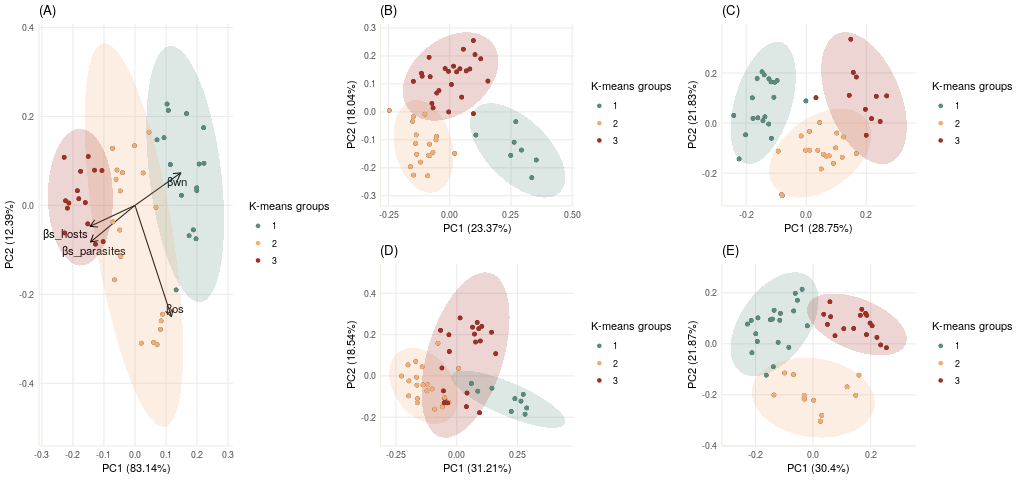
\includegraphics{figures/fig1.png}
\caption{Principal Component Analysis of networks beta-diversity metrics
and projection of local networks. For the dataset used here, networks
are described by three dimensions of beta-diversity: while
\emph{\(\beta\)s} captures part of the variation that is complementary
to that captured by \emph{\(\beta\)wn}, \emph{\(\beta\)os} describes a
completely different dimension of the data. (A) PCA of networks
beta-diversity metrics \emph{\(\beta\)s}, \emph{\(\beta\)wn} and
\emph{\(\beta\)os}; PCA of the phylogenetic component of PCD (PCDp) for
parasites (B) and hosts (C); PCA of the compositional component of PCD
(PCDc) for parasites (D) and hosts (E).}\label{fig:one}
}
\end{figure}

\hypertarget{each-beta-diversity-index-relates-in-a-particular-way-with-phylogenetically-community-dissimilarity-pcd.}{%
\subsubsection{Each beta-diversity index relates in a particular way
with phylogenetically community dissimilarity
(PCD).}\label{each-beta-diversity-index-relates-in-a-particular-way-with-phylogenetically-community-dissimilarity-pcd.}}

As expected, \emph{\(\beta\)s} and PCDc are proxies for each other both
for hosts and parasites, while PCDc is inversely correlated with
\emph{\(\beta\)wn} (fig.~\ref{fig:twoA}). Communities with a high
\emph{\(\beta\)s} value are very different from those around them, and
the change in species composition could also represent a shift in the
links inside these networks either because new species will probably
explore different ranges of ecological niche or because the loss of
species would also represent a loss of interaction. These changes in
links inside networks are represented by \emph{\(\beta\)os}, and its
relationship with both PCDc and PCDp is highly variable
(fig.~\ref{fig:twoB} and fig.~\ref{fig:threeB}).

Because any change in species composition highly affects phylogenetic
diversity, \emph{\(\beta\)s} is also positively correlated with PCDp
(fig.~\ref{fig:twoB}). Communities with high values for any of those
metrics are located in regions with expected higher biodiversity
(fig.~\ref{fig:threeA} and fig.~\ref{fig:threeB}), and this may indicate
that the biogeographical history of these communities are more related
to migration than diversification of local lineages (Davies and Buckley
2011). Therefore, networks with high PCDp also represent communities
with lower ecological redundancy and higher functional diversity because
it indicates that the species turnover is happening between species
phylogenetically distant.

On the other hand, networks that are better represented by
\emph{\(\beta\)wn} - i.e., those which differences between them are
significantly smaller than the differences in relation to the metaweb -
are also phylogenetically similar, varying always inside a limited range
of small dissimilarity (both with PCDc and PCDp). Because these
communities also have low values of \emph{\(\beta\)s}, indicating less
frequent species turnover, this dissimilarity is due to different links
between shared species. This result may reflect two possible
scenarios:\\
1. In similar communities with low phylogenetic diversity (shorter
branch lengths) the turnover of species could be adding very
ecologically similar lineages, which leads to different interactions to
prevent local extinction through competition.\\
2. In similar communities with high phylogenetic diversity (longer
branch lengths) the species turnover may have been a result of invasion
and migration, which may lead to opportunistic interactions.

This is also illustrated in fig.~\ref{fig:twoA} and fig.~\ref{fig:twoB}
on scatterplots of \emph{\(\beta\)os} vs.~PCD: networks that differ
little in phylogenies have a broader range of values of
\emph{\(\beta\)os}, while highly phylogenetically distinct networks only
have very low values of \emph{\(\beta\)os} - meaning that, for
communities with high values of PCD, the few species that are shared
interact in the same way. Additionally, because those same communities
also have low values of \emph{\(\beta\)wn} (i.e., they are very similar
to the overall metaweb) and high values of \emph{\(\beta\)s} (i.e., high
species turnover), the interactions are probably being conserved also
when species are replaced, like when two species that are
phylogenetically distant replace each other in the same ecological
function.

\begin{figure}
\hypertarget{fig:twoA}{%
\centering
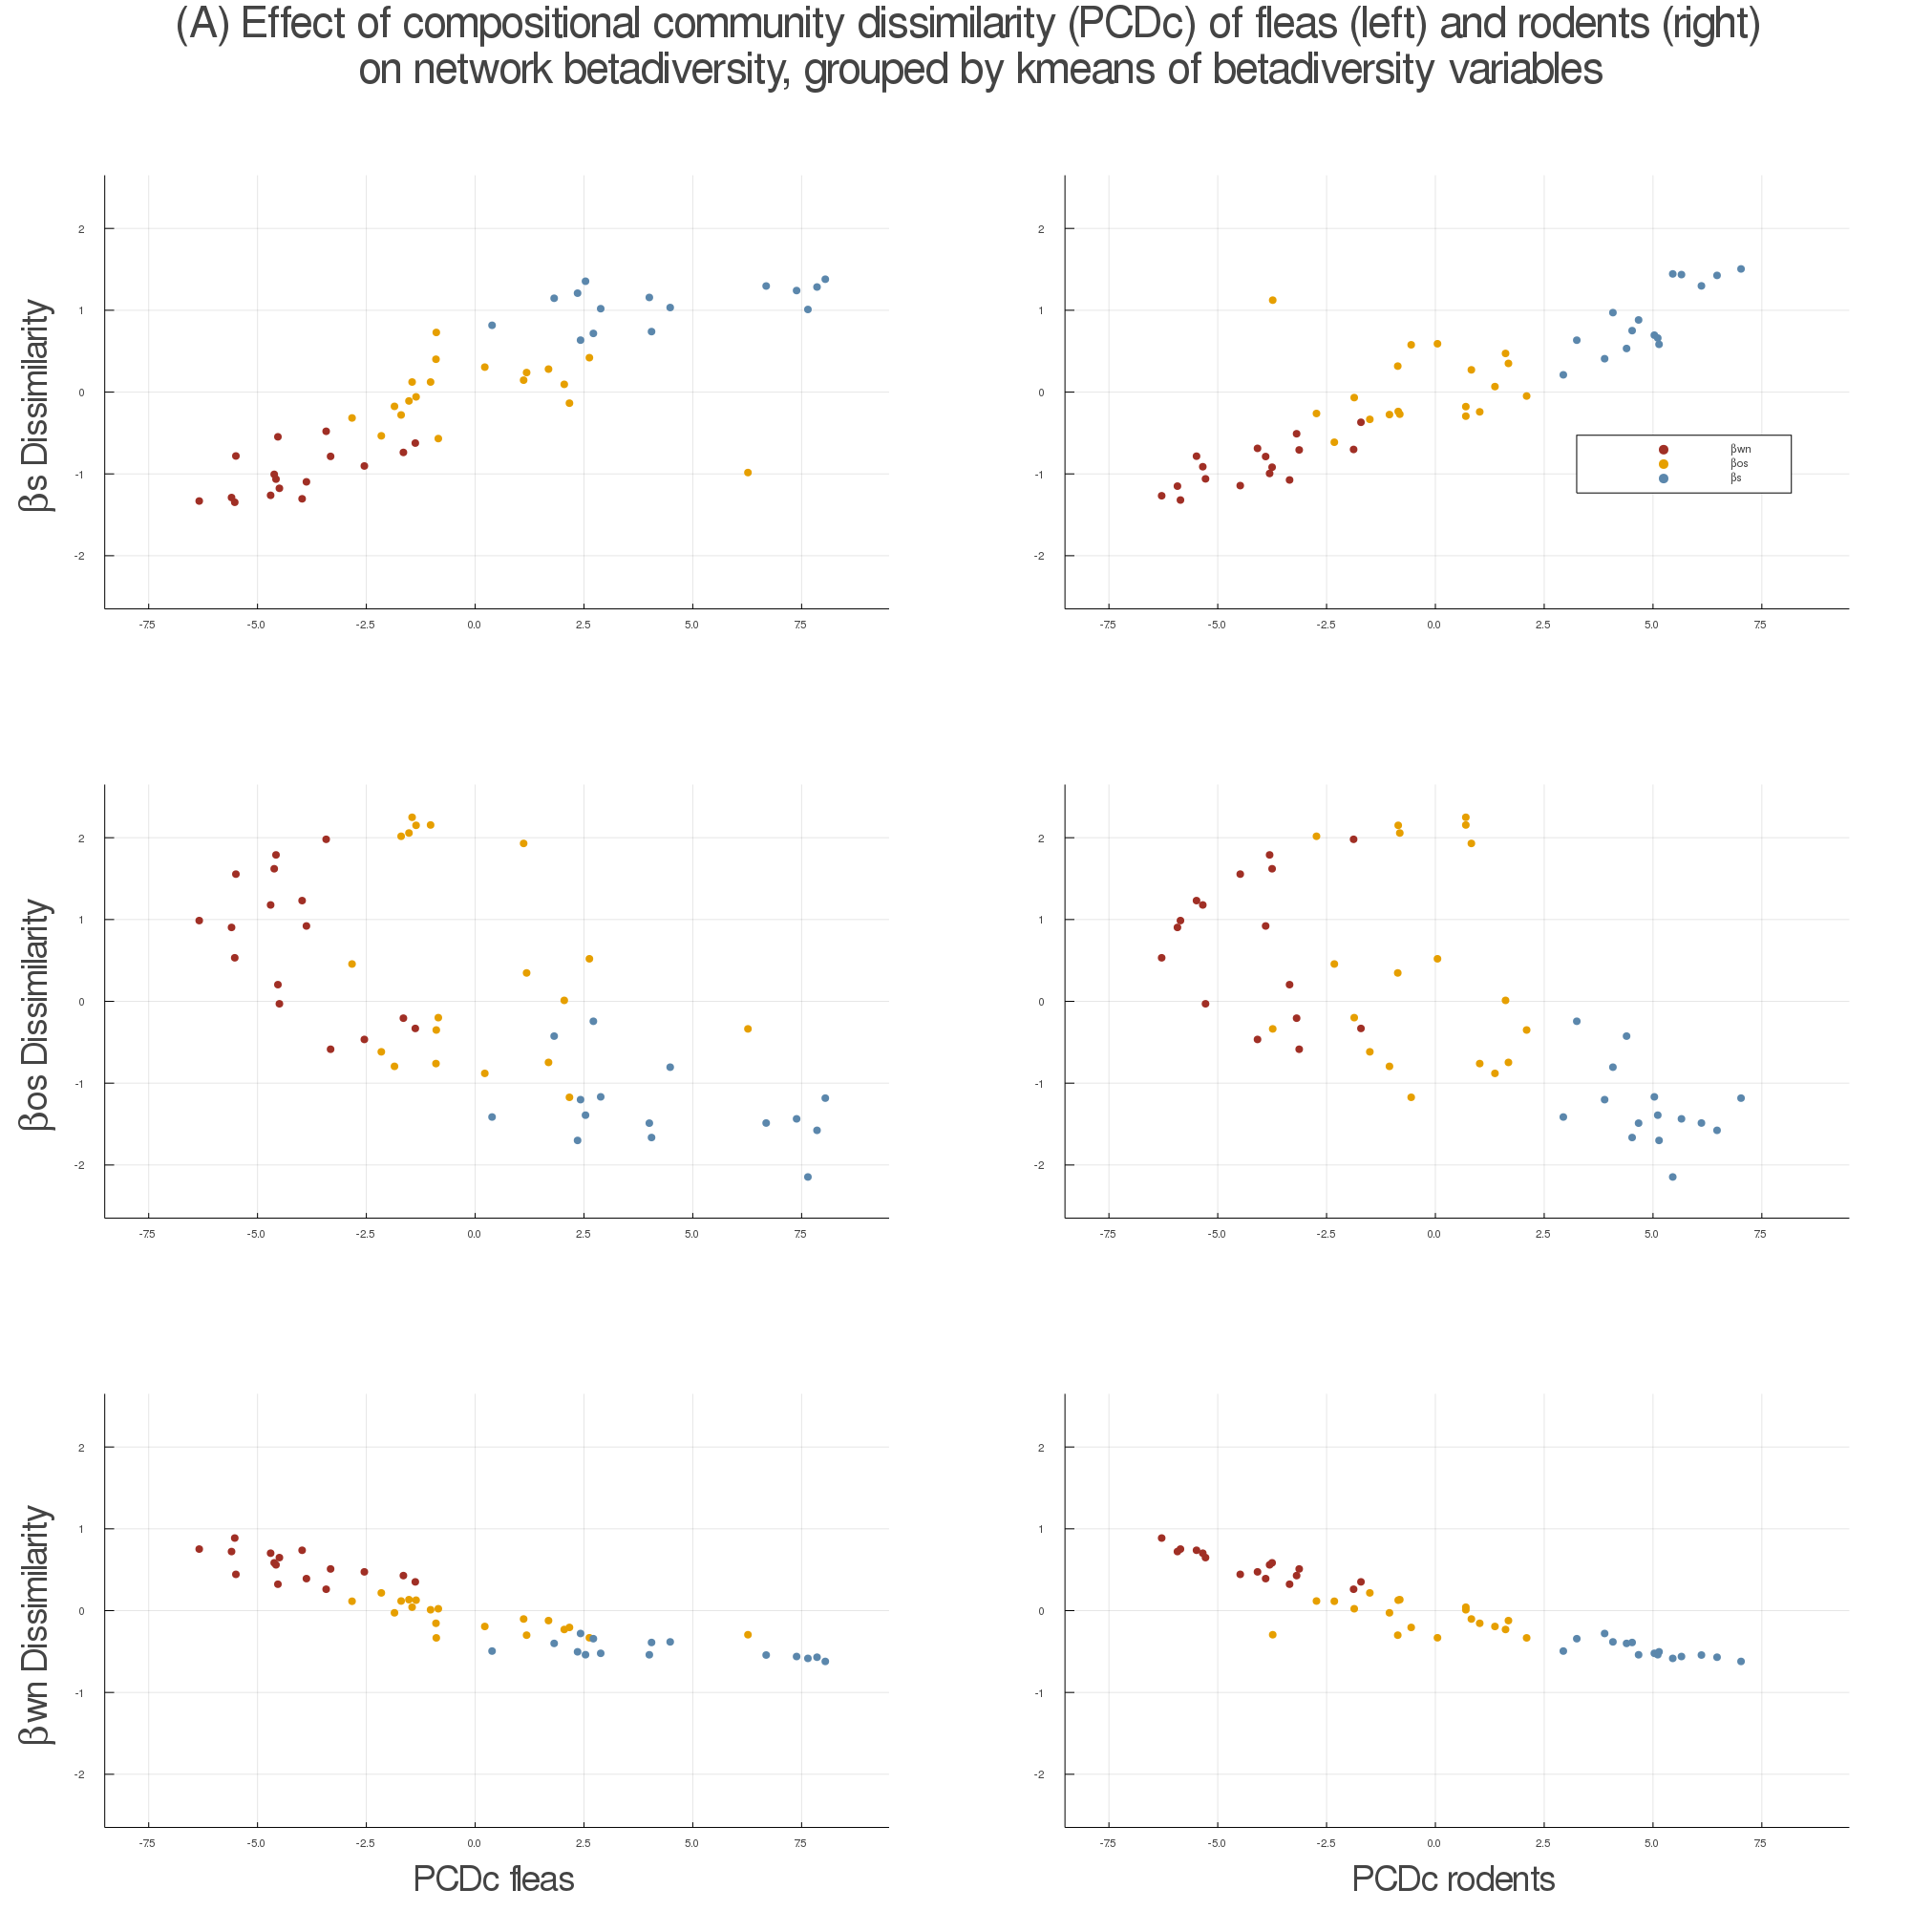
\includegraphics{figures/fig2A.png}
\caption{Effects of the compositional element of phylogenetic diversity
dissimilarity on network beta-diversity for both parasites (left) and
hosts (right). The colours correspond to the groups described on fig.~1.
Networks with higher values of PCDc are taxonomically more distinct and
therefore have higher values of \emph{\(\beta\)s} and lower values of
\emph{\(\beta\)os} because they do not share many
species.}\label{fig:twoA}
}
\end{figure}

\begin{figure}
\hypertarget{fig:twoB}{%
\centering
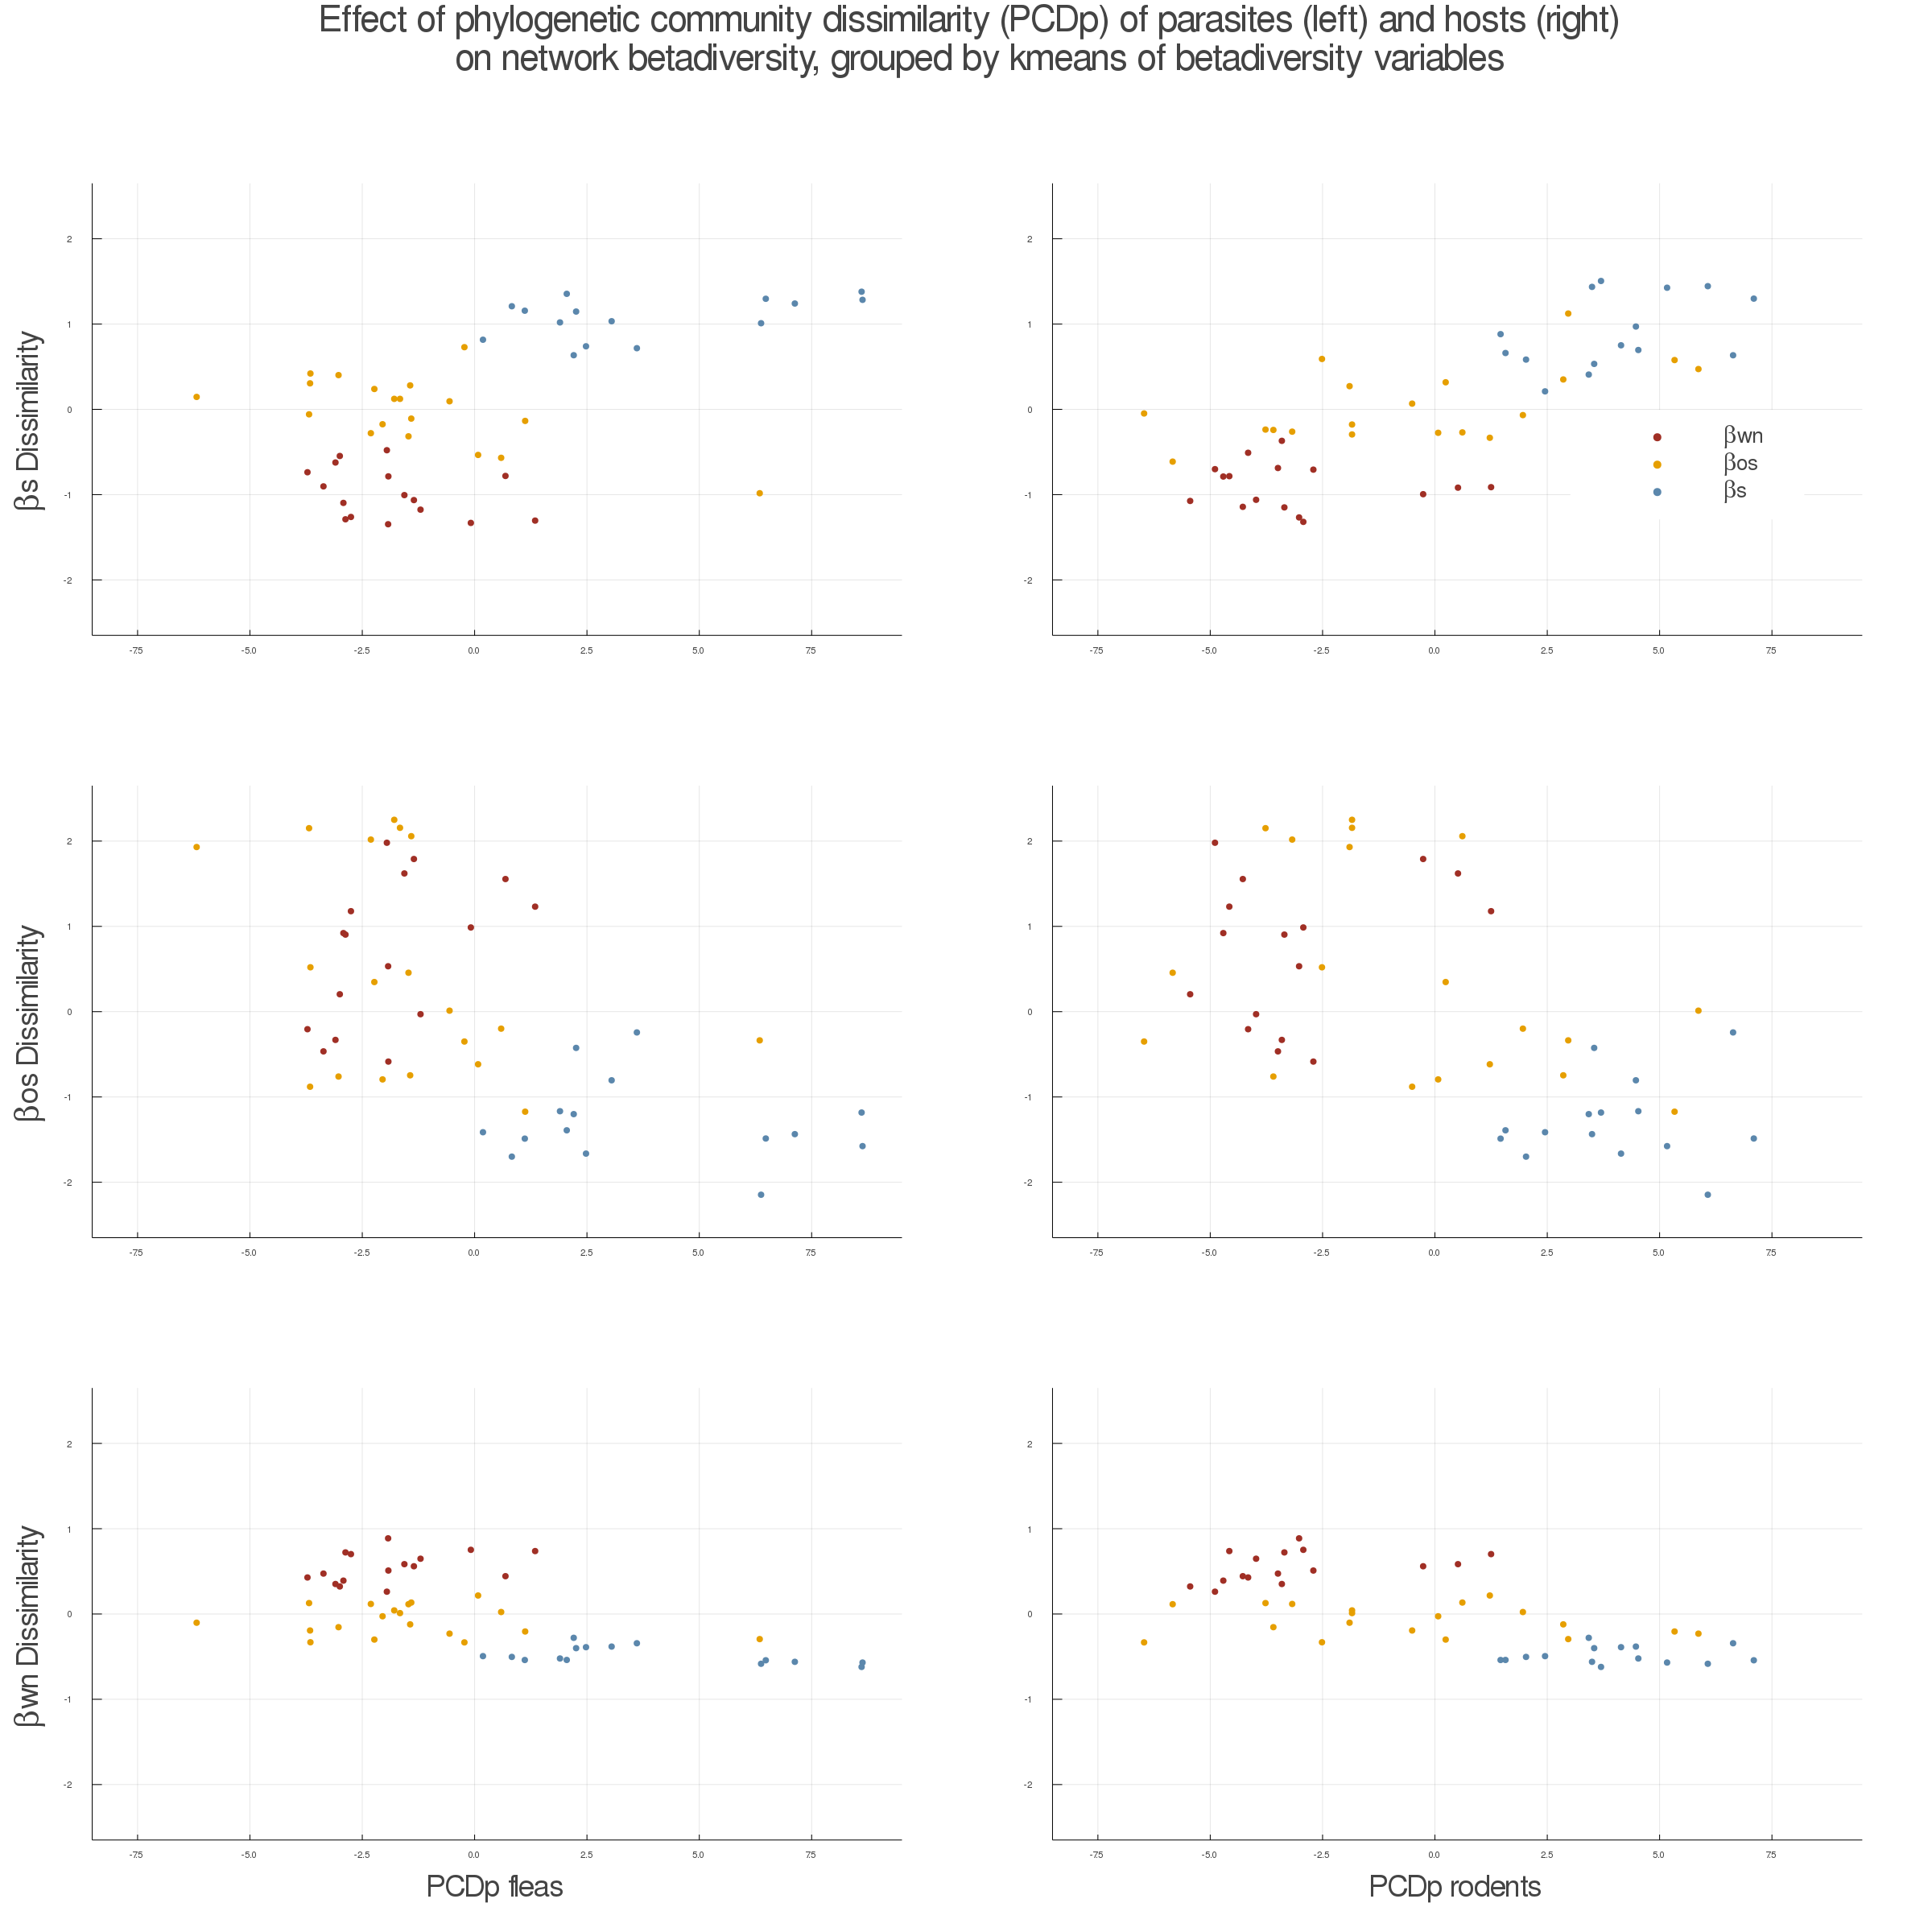
\includegraphics{figures/fig2B.png}
\caption{Effects of the phylogenetic component of the phylogenetic
diversity dissimilarity on network beta-diversity for both parasites
(left) and hosts (right). The colours correspond to the groups described
on fig.~1. Networks with higher values of PCDp are phylogenetically more
distinct, and therefore have lower values of \emph{\(\beta\)os} (because
they do not share many species). Networks better represented by
\emph{\(\beta\)wn} and \emph{\(\beta\)os} are less distinguished on this
aspect, but usually have lower values of PCDp.}\label{fig:twoB}
}
\end{figure}

\hypertarget{the-separation-of-communities-by-components-of-beta-diversity-was-also-observed-geographically}{%
\subsubsection{The separation of communities by components of
beta-diversity was also observed
geographically}\label{the-separation-of-communities-by-components-of-beta-diversity-was-also-observed-geographically}}

There is a gradual transition between networks that were better
described by turnover of species, clustered in central south Eurasia, to
those more unique compared to the metaweb, spread in the north
(fig.~\ref{fig:threeA}). The regional species pool is expected to be
more diverse towards the tropics, and therefore local networks have a
higher chance to have different species composition, which results in a
strong contribution of \emph{\(\beta\)s} for networks beta-diversity.
Because of the high diversity, species are functionally ``packed,'' and
although some species could have more generalist interactions, they
would rarely do so, in order to avoid competition. Heading north,
species turnover would be less frequent due to a decrease in regional
species richness, and now networks have more shared species. They start
to ``unpack'' and establish interactions with other remaining species,
and therefore the \emph{\(\beta\)os} component of beta-diversity
explains better why networks are different. The third group of networks,
characterized by a high value of \emph{\(\beta\)wn}, is also composed by
phylogenetically similar communities (as seen in fig.~\ref{fig:twoB}).
Because the species richness is even lower, any change in composition
can have a high impact on interactions. Therefore, the
\emph{\(\beta\)os} component is still very important, but now
differences in interactions due to species turnover contribute much more
to networks' beta-diversity.

The phylogenetic community dissimilarity of networks was also
geographically grouped, and in the region where \emph{\(\beta\)s} was
more important, there was a very distinguished group for both fleas' and
mammals' phylogenetic dissimilarity (fig.~\ref{fig:threeB}). The two
other groups are differently arranged in space: PCDc groups have a
similar latitudinal distribution, but different longitudinal ranges,
while PCDp groups are the opposite. This distribution of phylogenetic
groups highlight the uniqueness of the southern-central set of
communities, which suggests historical isolation of species.
Additionally, the purely phylogenetic component of PCD reinforces the
geographic distribution of beta-diversity metrics as seen in
fig.~\ref{fig:threeA}, with one group largely spread in the north -
occupying a diverse range of environments - and two other groups
restricted to latitudes under 60° (fig.~\ref{fig:threeB}).

\begin{figure}
\hypertarget{fig:threeA}{%
\centering
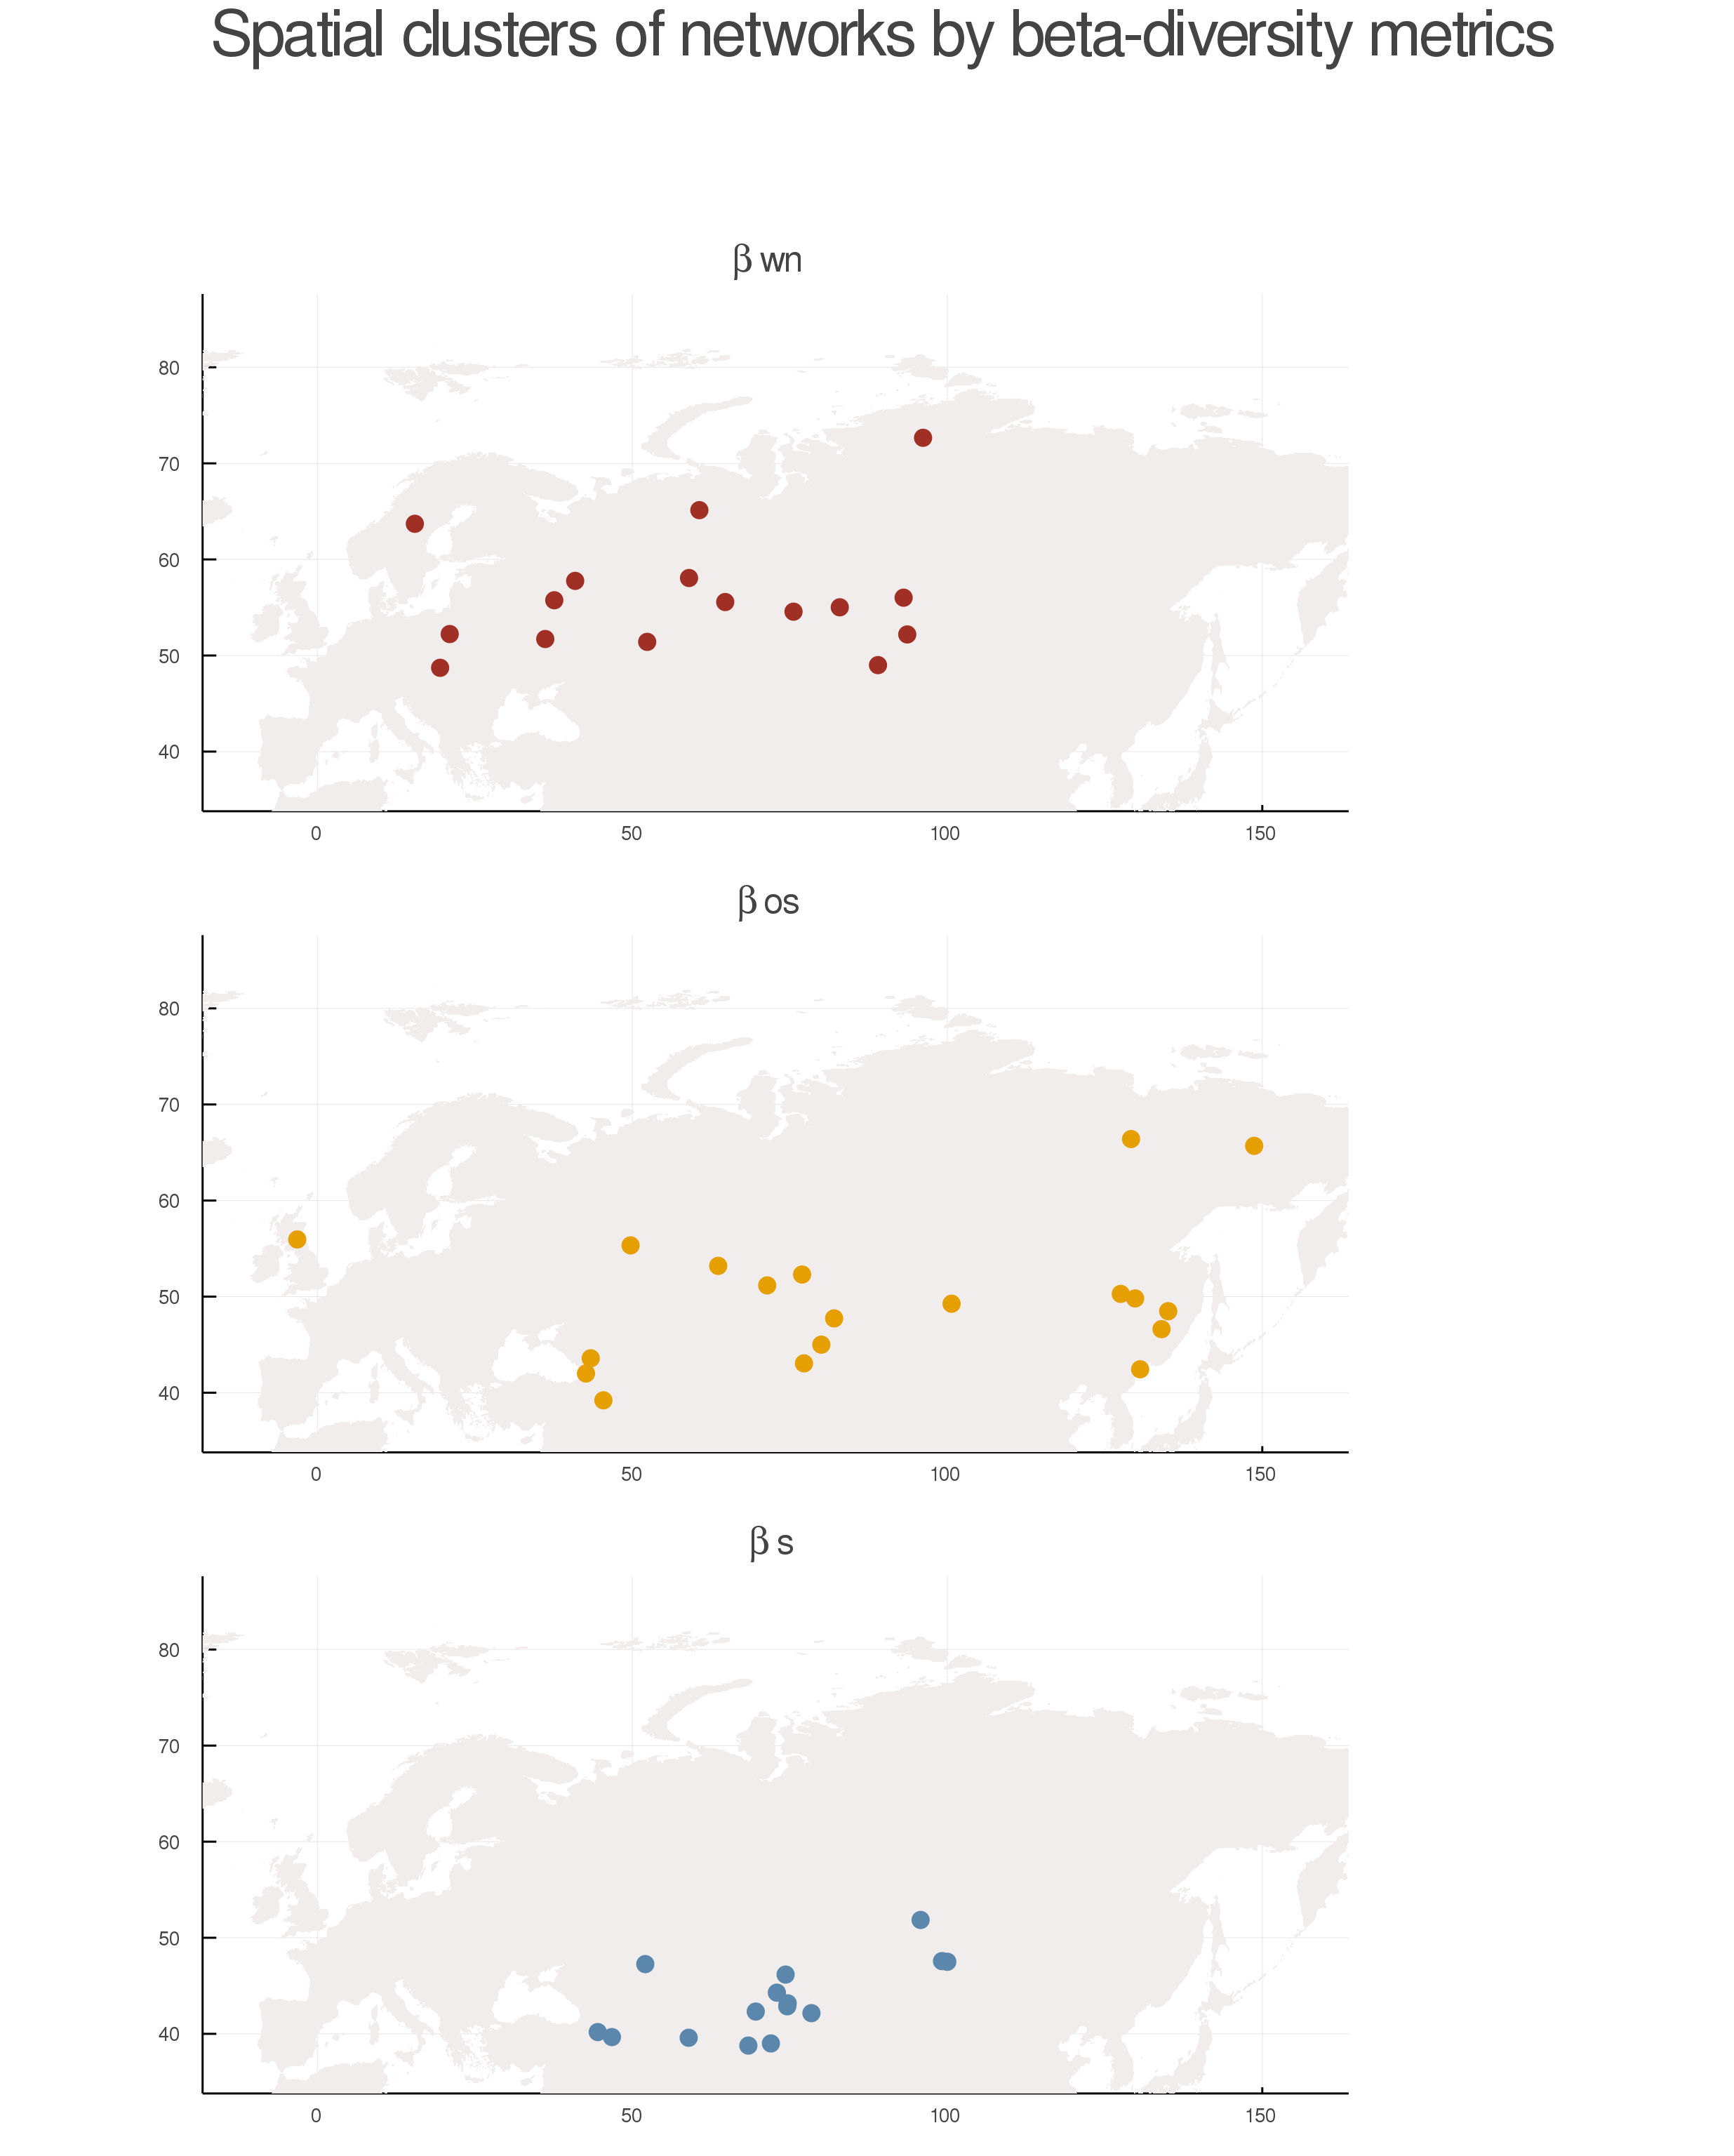
\includegraphics{figures/fig3A.png}
\caption{Spatial distribution of beta-diversity metrics. The groups
detected in fig.~1 are also geographically
distinguished}\label{fig:threeA}
}
\end{figure}

\begin{figure}
\hypertarget{fig:threeB}{%
\centering
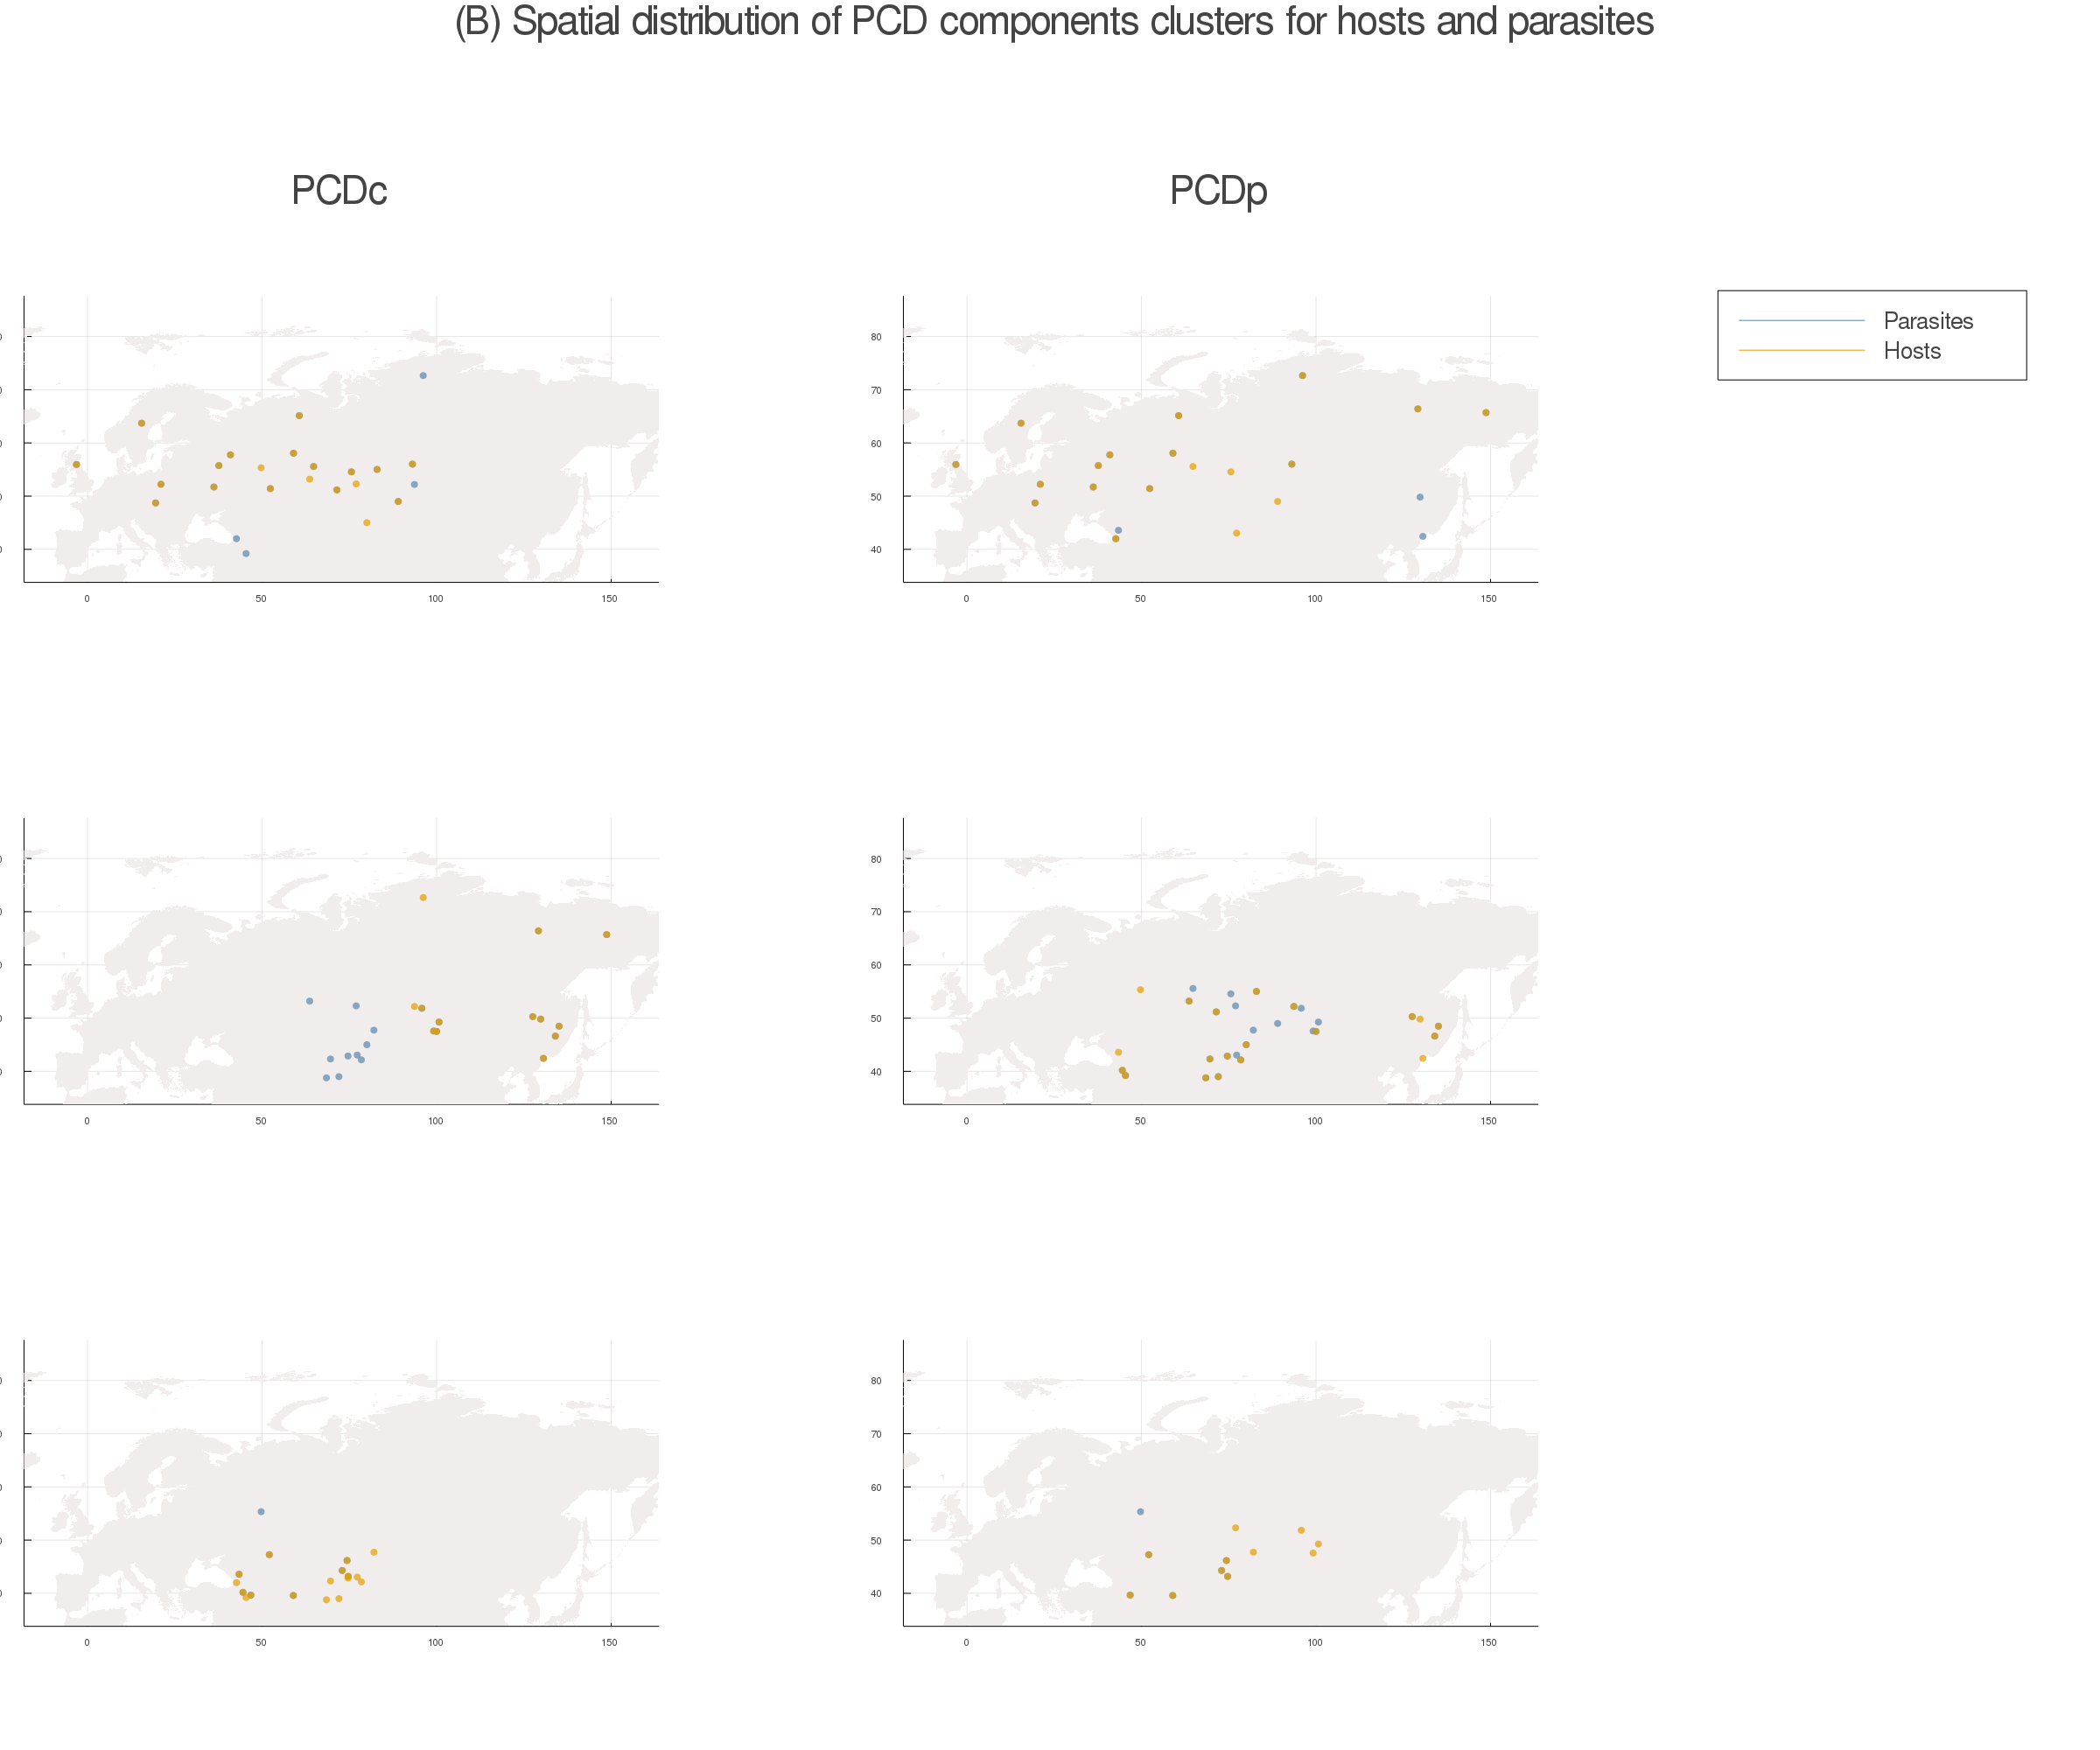
\includegraphics{figures/fig3B.png}
\caption{Spatial distribution of PCD components. Again, a distinct PCDc
cluster (as seen on the third map of the left column) matches the
cluster for which \emph{\(\beta\)s} metric is more
important.}\label{fig:threeB}
}
\end{figure}

\hypertarget{conclusion}{%
\subsection{Conclusion}\label{conclusion}}

The conspicuous association - both numerical and geographical - between
the evolutionary history of species and networks' beta-diversity
properties clarifies key aspects of the biogeography of hosts and
parasites communities in Eurasia. For example, the longitudinal PCDc
clusters separation roughly coincide with the presence of the Ural
Mountains. From this point of view, considering the longitudinal spread
of PCDp, the history of both hosts and parasites seems to follow a path
of migration and diversification from south-central Eurasia towards the
north. This history is also sustained by the metaweb beta-diversity
metrics: with a distinctive \emph{\(\beta\)s} group at the south of the
Ural Mountains suggesting higher species richness and common origin,
followed towards north by gradual changes in interactions and
composition, they sum up to the information unveiled by PCDp to describe
a very likely biogeographic history. By describing how the phylogenetic
differences between networks vary in the same way within groups, this
result seems to reinforce previous findings that there is no
co-phylogenetic matching between regional and local networks (Poisot and
Stouffer 2018). If networks co-varied in continental scale in the same
way they co-vary in local scale, our analyses would not detect the
groups illustrated in fig.~\ref{fig:threeB}.

Finally, this paper highlights how beta-diversity and phylogenetic
dissimilarity are related to each other, and sheds light on the
possibility that they interact with the environment in different ways.
While \emph{\(\beta\)s} seems to be connected to environmental
uniqueness and geographical barriers, \emph{\(\beta\)os} and
\emph{\(\beta\)wn} better reflect migration processes and evolutive
trajectories. As stated at the beginning of this text, ecological
networks are valuable, multidimensional lenses through which we can
investigate biodiversity and its history. Although we did not account
for properties such as phenology and natural history aspects of species,
we did find that small scale processes such as species interactions can
be integrated in large scale investigations and can have a stamp in
macroecological processes.

Interaction networks between parasites and hosts have great potential to
be used as study systems in the geographic variation of interactions
(Proulx, Promislow, and Phillips 2005; Poulin 2010). Because of the
particular type of association between parasites and hosts, the
dissimilarity of these interactions networks reflect not only the
environmental differences, but also the replacement of the host species
(Eriksson et al. 2019; Boris R. Krasnov et al. 2005; Poulin and Krasnov
2010). Nevertheless, the association between parasites and hosts is
often the result of the evolutionary history of the groups, and this
history can result in a non-neutral contribution of these species to the
beta diversity of these communities (Poisot et al. 2012). The underlying
logic of our approach pertains to a wide diversity of systems; not only
do rodents act as reservoirs for zoonotic diseases, (2020) show that
understanding the global-scale structure of host-virus interactions
\emph{requires} a joint understanding of the geographical and
evolutionary mechanisms involved in shaping them. We argue that when the
data are available, there is even more information to be gained by
looking at the way interactions vary.

\hypertarget{references}{%
\subsection*{References}\label{references}}
\addcontentsline{toc}{subsection}{References}

\hypertarget{refs}{}
\begin{CSLReferences}{1}{0}
\leavevmode\hypertarget{ref-Albery2020PreGlo}{}%
Albery, Gregory F., Evan A. Eskew, Noam Ross, and Kevin J. Olival. 2020.
{``Predicting the Global Mammalian Viral Sharing Network Using
Phylogeography.''} \emph{Nature Communications} 11 (1): 2260.
\url{https://doi.org/10.1038/s41467-020-16153-4}.

\leavevmode\hypertarget{ref-Baiser2019EcoRul}{}%
Baiser, Benjamin, Dominique Gravel, Alyssa R. Cirtwill, Jennifer A.
Dunne, Ashkaan K. Fahimipour, Luis J. Gilarranz, Joshua A. Grochow, et
al. 2019. {``Ecogeographical Rules and the Macroecology of Food Webs.''}
\emph{Global Ecology and Biogeography} 28 (9): 1204--18.
\url{https://doi.org/10.1111/geb.12925}.

\leavevmode\hypertarget{ref-Bezanson2017JulFre}{}%
Bezanson, Jeff, Alan Edelman, Stefan Karpinski, and Viral B Shah. 2017.
{``Julia: A Fresh Approach to Numerical Computing.''} \emph{SIAM Review}
59 (1): 65--98.

\leavevmode\hypertarget{ref-Bruder2017BioInt}{}%
Bruder, Andreas, Romana K Salis, Peter E Jones, and Christoph D
Matthaei. 2017. {``Biotic Interactions Modify Multiple-Stressor Effects
on Juvenile Brown Trout in an Experimental Stream Food Web.''}
\emph{Global Change Biology} 23 (9): 3882--94.
\url{https://doi.org/10.1111/gcb.13696}.

\leavevmode\hypertarget{ref-Canard2014EmpEva}{}%
Canard, E F, N Mouquet, D Mouillot, M Stanko, D Miklisova, and D Gravel.
2014. {``Empirical Evaluation of Neutral Interactions in Host-Parasite
Networks.''} \emph{The American Naturalist} 183 (4): 468--79.

\leavevmode\hypertarget{ref-CHAMuha2015EmpRes}{}%
Cha, Muha, Xiaodong Wu, Heping Fu, Shuai Yuan, Yunga Wu, and Xiaodong
Zhang. 2015. {``An Empirical Research of Rodent Metacommunities in
Alashan Desert.''} \emph{Acta Ecologica Sinica} 35 (17).
\url{https://doi.org/10.5846/stxb201312092913}.

\leavevmode\hypertarget{ref-Coelho2017NeuBio}{}%
Coelho, Marco Túlio Pacheco, João Fabrício Mota Rodrigues, and Thiago F
Rangel. 2017. {``Neutral Biogeography of Phylogenetically Structured
Interaction Networks.''} \emph{Ecography} 40 (12): 1467--74.

\leavevmode\hypertarget{ref-Dalsgaard2013HisCli}{}%
Dalsgaard, Bo, Kristian Trøjelsgaard, Ana M Martín González, David
Nogués-Bravo, Jeff Ollerton, Theodora Petanidou, Brody Sandel, et al.
2013. {``Historical Climate-Change Influences Modularity and Nestedness
of Pollination Networks.''} \emph{Ecography} 36 (12): 1331--40.

\leavevmode\hypertarget{ref-Davies2011PhyDiv}{}%
Davies, T Jonathan, and Lauren B Buckley. 2011. {``Phylogenetic
Diversity as a Window into the Evolutionary and Biogeographic Histories
of Present-Day Richness Gradients for Mammals.''} \emph{Philos. Trans.
R. Soc. Lond. B Biol. Sci.} 366 (1576): 2414--25.

\leavevmode\hypertarget{ref-Desdevises2015ComAna}{}%
Desdevises, Yves, Serge Morand, Boris R. Krasnov, and Julien Claude.
2015. {``Comparative Analysis: Recent Developments and Uses with
Parasites.''} In \emph{Parasite Diversity and Diversification:
Evolutionary Ecology Meets Phylogenetics}, edited by Serge Morand, Boris
R. Krasnov, and D. Timothy J. Littlewood, 337--50. Cambridge: Cambridge
University Press. \url{https://doi.org/10.1017/CBO9781139794749.023}.

\leavevmode\hypertarget{ref-Doxford2013SpaTem}{}%
Doxford, Simon W., Mark K. J. Ooi, and Robert P. Freckleton. 2013.
{``Spatial and Temporal Variability in Positive and Negative
Plant-Bryophyte Interactions Along a Latitudinal Gradient.''}
\emph{Journal of Ecology} 101 (2): 465--74.
\url{https://doi.org/10.1111/1365-2745.12036}.

\leavevmode\hypertarget{ref-Eriksson2019HosEnv}{}%
Eriksson, Alan, Jean-françois Doherty, Erich Fischer, Gustavo Graciolli,
and Robert Poulin. 2019. {``Hosts and Environment Overshadow Spatial
Distance as Drivers of Bat Fly Species Composition in the Neotropics.''}
\emph{Journal of Biogeography}.

\leavevmode\hypertarget{ref-Gravel2019BriElt}{}%
Gravel, Dominique, Benjamin Baiser, Jennifer A. Dunne, Jens-Peter
Kopelke, Neo D. Martinez, Tommi Nyman, Timothée Poisot, et al. 2019.
{``Bringing Elton and Grinnell Together: A Quantitative Framework to
Represent the Biogeography of Ecological Interaction Networks.''}
\emph{Ecography} 42 (3): 401--15.
\url{https://doi.org/10.1111/ecog.04006}.

\leavevmode\hypertarget{ref-Hadfield2014-tw}{}%
Hadfield, Jarrod D, Boris R Krasnov, Robert Poulin, and Shinichi
Nakagawa. 2014. {``A Tale of Two Phylogenies: Comparative Analyses of
Ecological Interactions.''} \emph{The American Naturalist} 183 (2):
174--87.

\leavevmode\hypertarget{ref-Hadfield2013DatTal}{}%
Hadfield, Jarrod D, Boris R Krasnov, Robert Poulin, and Nakagawa
Shinichi. 2013. {``Data from: A Tale of Two Phylogenies: Comparative
Analyses of Ecological Interactions.''}
\url{https://doi.org/10.5061/DRYAD.JF3TJ}.

\leavevmode\hypertarget{ref-Holt2002FooWeb}{}%
Holt, Robert D. 2002. {``Food Webs in Space: On the Interplay of Dynamic
Instability and Spatial Processes.''} \emph{Ecological Research} 17 (2):
261--73. \url{https://doi.org/10.1046/j.1440-1703.2002.00485.x}.

\leavevmode\hypertarget{ref-Kaplan2005AphAlt}{}%
Kaplan, Ian, and Micky D. Eubanks. 2005. {``Aphids Alter the
Community-Wide Impact of Fire Ants.''} \emph{Ecology} 86 (6): 1640--49.
\url{https://doi.org/10.1890/04-0016}.

\leavevmode\hypertarget{ref-Koleff2003MeaBet}{}%
Koleff, Patricia, Kevin J Gaston, and Jack J Lennon. 2003. {``Measuring
Beta Diversity for Presence-Absence Data.''} \emph{Journal of Animal
Ecology} 72 (3): 367--82.

\leavevmode\hypertarget{ref-Konig2014ConRes}{}%
König, Malin A. E., Christer Wiklund, and Johan Ehrlén. 2014.
{``Context-Dependent Resistance Against Butterfly Herbivory in a
Polyploid Herb.''} \emph{Oecologia} 174 (4): 1265--72.
\url{https://doi.org/10.1007/s00442-013-2831-4}.

\leavevmode\hypertarget{ref-Krasnov2015PhySig}{}%
Krasnov, Boris R., Serge Morand, and Robert Poulin. 2015.
{``Phylogenetic Signals in Ecological Properties of Parasites.''} In
\emph{Parasite Diversity and Diversification: Evolutionary Ecology Meets
Phylogenetics}, edited by Serge Morand, Boris R. Krasnov, and D. Timothy
J. Littlewood, 351--59. Cambridge: Cambridge University Press.
\url{https://doi.org/10.1017/CBO9781139794749.024}.

\leavevmode\hypertarget{ref-Krasnov2005SpaVar}{}%
Krasnov, Boris R, Georgy I Shenbrot, David Mouillot, Irina S Khokhlova,
and Robert Poulin. 2005. {``Spatial Variation in Species Diversity and
Composition of Flea Assemblages in Small Mammalian Hosts: Geographical
Distance or Faunal Similarity?''} \emph{Journal of Biogeography} 32 (4):
633--44.

\leavevmode\hypertarget{ref-Li2020PhyRP}{}%
Li, Daijiang, Russell Dinnage, Lucas Nell, Matthew R. Helmus, and
Anthony Ives. 2020. {``Phyr: An R Package for Phylogenetic
Species-Distribution Modelling in Ecological Communities.''}
\emph{bioRxiv}. \url{https://doi.org/10.1101/2020.02.17.952317}.

\leavevmode\hypertarget{ref-Muola2010AssPla}{}%
Muola, Anne, Pia Mutikainen, Marianna Lilley, Liisa Laukkanen, Juha
Pekka Salminen, and Roosa Leimu. 2010. {``Associations of Plant Fitness,
Leaf Chemistry, and Damage Suggest Selection Mosaic in Plant-Herbivore
Interactions.''} \emph{Ecology}.
\url{https://doi.org/10.1890/09-0589.1}.

\leavevmode\hypertarget{ref-Poisot2020EcoMan}{}%
Poisot, Timothée, Francis Banville, and Gabriel Dansereau. 2020.
{``EcoJulia/Mangal.jl: V0.3.1.''} Zenodo.
\url{https://doi.org/10.5281/zenodo.4299306}.

\leavevmode\hypertarget{ref-Poisot2012DisSpe}{}%
Poisot, Timothée, Elsa Canard, David Mouillot, Nicolas Mouquet, and
Dominique Gravel. 2012. {``The Dissimilarity of Species Interaction
Networks.''} \emph{Ecology Letters} 15 (12): 1353--61.

\leavevmode\hypertarget{ref-Poisot2016StrPro}{}%
Poisot, Timothée, Alyssa R Cirtwill, Kévin Cazelles, Dominique Gravel,
Marie Josée Fortin, and Daniel B Stouffer. 2016. {``The Structure of
Probabilistic Networks.''} \emph{Methods in Ecology and Evolution} 7
(3): 303--12. \url{https://doi.org/10.1111/2041-210X.12468}.

\leavevmode\hypertarget{ref-Poisot2017HosPar}{}%
Poisot, Timothée, Cynthia Guéveneux-Julien, Marie Josée Fortin,
Dominique Gravel, and Pierre Legendre. 2017. {``Hosts, Parasites and
Their Interactions Respond to Different Climatic Variables.''}
\emph{Global Ecology and Biogeography} 26 (8): 942--51.
\url{https://doi.org/10.1111/geb.12602}.

\leavevmode\hypertarget{ref-Poisot2020EcoNet}{}%
Poisot, Timothée, Michiel Stock, Laura Hoebeke, Piotr Szefer, Francis
Banville, and Giulio V. Dalla Riva. 2020. {``Ecological Networks
Analyses in Julia.''} Zenodo.
\url{https://doi.org/10.5281/zenodo.4302247}.

\leavevmode\hypertarget{ref-Poisot2018IntRet}{}%
Poisot, Timothée, and Daniel B. Stouffer. 2018. {``Interactions Retain
the Co-Phylogenetic Matching That Communities Lost.''} \emph{Oikos} 127
(2): 230--38. \url{https://doi.org/10.1111/oik.03788}.

\leavevmode\hypertarget{ref-Poisot2014SpeWhy}{}%
Poisot, Timothée, Daniel B. Stouffer, and Dominique Gravel. 2014.
{``Beyond Species: Why Ecological Interaction Networks Vary Through
Space and Time.''} \emph{Oikos} 124 (3): 243--51.
\url{https://doi.org/10.1111/oik.01719}.

\leavevmode\hypertarget{ref-Poulin2010NetAna}{}%
Poulin, Robert. 2010. {``Network Analysis Shining Light on Parasite
Ecology and Diversity.''} \emph{Trends in Parasitology} 26 (10):
492--98. \url{https://doi.org/10.1016/j.pt.2010.05.008}.

\leavevmode\hypertarget{ref-Poulin2010SimVar}{}%
Poulin, Robert, and Boris R Krasnov. 2010. {``Similarity and Variability
of Parasite Assemblage Across Geographical Space.''} In \emph{The
Biogeography of Host-Parasite Interactions}, edited by Serge Morand and
Boris R Krasnov, 115127. Great Claredon Street, Oxford: Oxford
University Press.

\leavevmode\hypertarget{ref-Proulx2005NetThi}{}%
Proulx, S, D Promislow, and P Phillips. 2005. {``Network Thinking in
Ecology and Evolution.''} \emph{Trends in Ecology \& Evolution} 20 (6):
345--53. \url{https://doi.org/10.1016/j.tree.2005.04.004}.

\leavevmode\hypertarget{ref-RCoreTeam2018RLan}{}%
R Core Team. 2018. \emph{R: A Language and Environment for Statistical
Computing}. Manual. Vienna, Austria: R Foundation for Statistical
Computing.

\leavevmode\hypertarget{ref-Rall2012UniTem}{}%
Rall, B. C., U. Brose, M. Hartvig, G. Kalinkat, F. Schwarzmuller, O.
Vucic-Pestic, and O. L. Petchey. 2012. {``Universal Temperature and
Body-Mass Scaling of Feeding Rates.''} \emph{Philosophical Transactions
of the Royal Society B: Biological Sciences} 367 (1605): 2923--34.
\url{https://doi.org/10.1098/rstb.2012.0242}.

\leavevmode\hypertarget{ref-Sebastian-Gonzalez2015MacTre}{}%
Sebastián-González, Esther, Bo Dalsgaard, Brody Sandel, and Paulo R
Guimarães. 2015. {``Macroecological Trends in Nestedness and Modularity
of Seed-Dispersal Networks: Human Impact Matters.''} \emph{Global
Ecology and Biogeography} 24 (3): 293--303.

\leavevmode\hypertarget{ref-Trojelsgaard2013MacPol}{}%
Trøjelsgaard, Kristian, and Jens M Olesen. 2013. {``Macroecology of
Pollination Networks.''} \emph{Global Ecology and Biogeography} 22 (2):
149--62.

\leavevmode\hypertarget{ref-Tylianakis2017EcoNet}{}%
Tylianakis, Jason M., and Rebecca J. Morris. 2017. {``Ecological
Networks Across Environmental Gradients.''} \emph{Annual Review of
Ecology, Evolution, and Systematics} 48 (1):
annurev-ecolsys-110316-022821.
\url{https://doi.org/10.1146/annurev-ecolsys-110316-022821}.

\end{CSLReferences}

\end{document}
